\documentclass[../differential_geometry.tex]{subfiles}
\begin{document}
\section{Aula 10 - 09 de Abril, 2026}
\subsection{Motivações}
\begin{itemize}
	\item Plano Tangente;
	\item A Primeira Forma Fundamental;
	\item Plano Hiperbólico.
\end{itemize}
\subsection{Plano Tangente}
Na última aula, enunciamos a proposição que caracteriza o plano tangente:
\begin{prop*}
	Seja \(\underline{x}:U\subseteq \mathbb{R}^{2}\rightarrow S\) uma parametrização local de S e q um ponto de U. Então, o plano \(\mathrm{d}\underline{x}_{q}(\mathbb{R}^{2})\) coincide com o espaço de todos os vetores tangente a s no ponto \(p = \underline{x}(q)\).
\end{prop*}
\begin{proof*}
	Precisamos mostrar que
	\[
		\mathrm{d}\underline{x}_{q}(\mathbb{R}^{2})=\{a\underline{x}_{u}(q) + b \underline{x}_{v}(q):\; a, b\in \mathbb{R}\} = \{w:\; w\text{ é tangente a S em p}\}.
	\]
	\begin{figure}[H]
		\begin{center}
			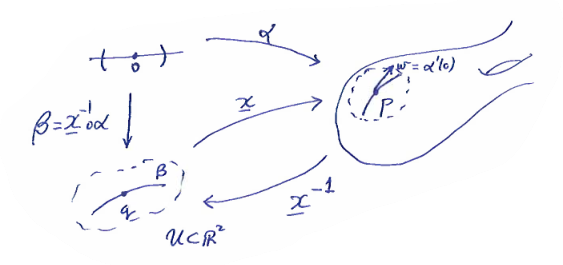
\includegraphics[height=\textheight, width=\textwidth, keepaspectratio]{./Images/proposition_09.png}
		\end{center}
	\end{figure}

	\(\tikz[baseline=-0.5ex]\draw[black, fill=black, radius=1.5pt](0, 0)circle;\; \subseteq \): seja w um ponto na imagem de \(\mathbb{R}^{2}\) por \(\mathrm{d}\underline{x}_{q}\), tal que \(w = \mathrm{d}x_{q}(v)\), com \(v\in \mathbb{R}^{2}\), e seja \(\beta(t) = q + tv\), onde t é pequeno, uma parametrização do segmento de reta em U, passando por q e paralelo a v:
	\begin{figure}[H]
		\begin{center}
			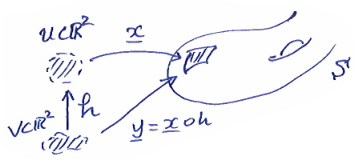
\includegraphics[height=0.7\textheight, width=0.7\textwidth, keepaspectratio]{./Images/reparametrization_09.png}
		\end{center}
	\end{figure}

	Definindo uma curva \(\alpha (t) = \underline{x}(q+tv)\subseteq S\) em S com \(\alpha (0) = p\), temos \(\alpha'(0) = \mathrm{d}\underline{x}_{q}(v) = w\), e portanto
	\[
		\mathrm{d}\underline{x}_{q}(\mathbb{R}^{2})\subseteq \{w:\; w \text{ é um vetor tangente a S em p}\}.
	\]

	\(\tikz[baseline=-0.5ex]\draw[black, fill=black, radius=1.5pt](0, 0)circle;\; \supseteq \): vamos aceitar que a aplicação \(\underline{x}^{-1}:x(U)\rightarrow \mathbb{R}^{2}\) é suave. Feito isso, considere w um vetor tangente a S em p; então, existe uma curva regular \(\alpha :(-\varepsilon , \varepsilon )\rightarrow S\) com \(\alpha (0) = p\) e \(\alpha '(0) = w\)

	Considere, agora, \(\beta :(-\varepsilon , \varepsilon )\rightarrow U\subseteq \mathbb{R}^{2}\) dada por
	\[
		\beta (t) = (\underline{x}^{-1}\circ \alpha )(t) = \underline{x}^{-1}(\alpha (t));
	\]
	com isso,
	\[
		\mathrm{d}\underline{x}_{q}(\beta'(0)) = \frac{\mathrm{d}}{\mathrm{d}t}(\underline{x}\circ \beta(t) )\biggl|_{\mathrlap{t=0}}^{}\biggr. = \frac{\mathrm{d}}{\mathrm{d}t}(\underline{x}\circ \underline{x}^{-1}\circ \alpha )(t)\biggl|_{\mathrlap{t=0}}^{}\biggr. = \alpha '(0) = w,
	\]
	e concluímos que \(w\in \mathrm{d}\underline{x}_{q}(\mathbb{R}^{2})\).

	Portanto, provamos a relação de continência dos dois lados. \qedsymbol
\end{proof*}
\begin{tcolorbox}[
		skin=enhanced,
		title=Observação,
		fonttitle=\bfseries,
		colframe=black,
		colbacktitle=cyan!75!white,
		colback=cyan!15,
		colbacklower=black,
		coltitle=black,
		drop fuzzy shadow,
		%drop large lifted shadow
	]
	Podemos concluir, também, que \(\mathrm{d}\underline{x}_{q}(\mathbb{R}^{2})\) não depende da parametrização local de \(\underline{x}\) de S em p!
\end{tcolorbox}

\begin{def*}
	O plano \(\mathrm{d}\underline{x}_{q}(\mathbb{R}^{2})\) é chamado \textbf{plano tangente a S no ponto p}, denotado por \(T_{p}S.\; \square\)
\end{def*}

Vimos acima que, para w em \(T_{p}S\), existe uma curva regular \(\beta :(-\varepsilon , \varepsilon )\rightarrow U \subseteq \mathbb{R}^{2}\) com \(\beta (0) = q\) e \(w = \mathrm{d}\underline{x}_{q}(\beta '(0))\).
A partir disso, poderemos determinar uma forma para w em coordenadas: nas condições exigidas, \(\beta (t)\) pode ser escrita como
\[
	\beta (t) = (u(t), v(t)),\; t \in (-\varepsilon , \varepsilon ) \quad\&\quad \beta '(0) = (u'(0), v'(0)).
\]
Logo,
\begin{align*}
	w = \mathrm{d}\underline{x}_{q}(\beta '(0)) & = \frac{\mathrm{d}}{\mathrm{d}t}((x\circ \beta )(t))\biggl|_{t=0}^{}\biggr. \\
	                                            & = \frac{\mathrm{d}}{\mathrm{d}t}x(u(t), v(t))\biggl|_{t=0}^{}\biggr.        \\
	                                            & = u'(0) \underline{x}_{u}(q) + v'(0) \underline{x}_{v}(q),
\end{align*}
permitindo escrevermos w com as coordenadas \((u'(0), v'(0))\) na base \(\{\underline{x}_{u}(q), \underline{x}_{v}(q)\}\) de \(T_{p}S\).

\begin{example}
	Seja \(g:U \subseteq \mathbb{R}^{2}\rightarrow \mathbb{R}\) uma função suave e
	\[
		S = \Gamma (g) = \{(u, v, g(u, v)):\; (u, v)\in U\}.
	\]
	Temos \(\underline{x}(u, v) = (u, v, g(u, v))\) é uma parametrização de S e, além disso, o plano tangente é
	\[
		T_{p}S = \mathbb{R}\cdot \{(1, 0, g_{u}(u, v)), (0, 1, g_{v}(u, v))\},\; p = \underline{x}(u, v).
	\]
\end{example}
\begin{example}
	Seja \(S = f^{-1}(c)\), onde c é um valor regular de \(f:\mathbb{R}^{3}\rightarrow \mathbb{R}\), e seja p um ponto de S; então, o plano tangente \(T_{p}S\) é ortogonal ao gradiente \(\nabla f(p) = (f_{x}(p), f_{y}(p), f_{z}(p))\) de f em p.

	Com efeito, seja \(\alpha :(-\varepsilon , \varepsilon )\rightarrow S\) uma curva regular com \(\alpha (0) = p\), tal que
	\[
		f(\alpha (t)) = c,\quad \forall t\in (-\varepsilon , \varepsilon ).
	\]
	Portanto, \(\nabla f(p)\) é ortogonal a \(\alpha '(0)\), ou seja,
	\[
		\nabla f(p)\cdot \alpha '(0) = 0'
	\]
\end{example}

\subsection{A Primeira Forma Fundamental}
No espaço euclidiano \(\mathbb{R}^{n}\), temos algumas propriedades e possibilidades bem legais! Por exemplo, podemos:
\begin{itemize}
	\item Medir a distância entre dois pontos A e B com \(d(A, B) = \sqrt[]{\langle \vec{AB}, \vec{AB} \rangle};\)
	\item Calcular o ângulo entre dois vetores com a relação \(\displaystyle \cos^{}{\theta } = \frac{\langle u, v \rangle}{\Vert u \Vert\Vert v \Vert}\);
	\item Calcular área de paralelogramos,
\end{itemize}
entre outras coisas. Todas as contas acima são feitas usando o produto escalar com o qual \(\mathbb{R}^{n}\) está munido, e queremos fazer tais contas em superfícies \(S\subseteq \mathbb{R}^{n}\) em particular, queremos calcular o \textit{comprimento de curvas em S}, o \textit{ângulo entre curvas em S} e a \textit{área de regiões em S}.

Pedimos que p seja um ponto de S e consideramos a restrição do produto escalar de \(\mathbb{R}^{n}\) a \(T_{p}S\), pois S não é, em geral, um subespaço vetorial de \(\mathbb{R}^{n}\), mas \(T_{p}S\) é; denotaremos a restrição imposta por \(\langle \cdot , \cdot  \rangle_{p}\).
Seja \(\underline{x}:U \subseteq \mathbb{R}^{2}\rightarrow S \subseteq \mathbb{R}^{n}\) uma parametrização local de S e \(p = \underline{x}(q)\), tal que
\[
	T_{p}S = \mathbb{R}\cdot \{\underline{x}_{u}(q), \underline{x}_{v}(q)\}.
\]
Daí, consideramos dois vetores \(w_1, w_2\in T_{p}S\) com
\[
	w_1 = a\underline{x}_{u}(q) + b \underline{x}_{v}(q)
\]
e
\[
	w_2 = c\underline{x}_{u}(q) + d \underline{x}_{v}(q).
\]
Com isso, podemos abrir a conta do produto interno:
\begin{align*}
	\langle w_1, w_2 \rangle_{p} & = \langle w_1, w_2 \rangle                                                                                                                                                                          \\
	                             & = \langle a\underline{x}_{u}(q) + b \underline{x}_{v}(q), c\underline{x}_{u}(q) + d \underline{x}_{v}(q) \rangle                                                                                    \\
	                             & = ac \langle \underline{x}_{u}(q), \underline{x}_{u}(q) \rangle + (ad+bc)\langle \underline{x}_{u}(q), \underline{x}_{v}(q) \rangle + bd \langle \underline{x}_{v}(q), \underline{x}_{v}(q) \rangle
\end{align*}
Logo, concluímos que a aplicação \(\langle \cdot , \cdot  \rangle_{p}:T_{p}S \times T_{p}S\rightarrow \mathbb{R}\) é bilinear, positiva e não degenerada -- é um produto escalar mesmo em \(T_{p}S\)!

\begin{def*}
	A forma quadrática \(I_{p}:T_{p}S\rightarrow \mathbb{R}\) dada por
	\[
		I_{p}(w)\coloneqq \langle w, w \rangle_{p}
	\]
	é chamada \textbf{primeira forma fundamental}. \(\square\)
\end{def*}
Se denotarmos os produtos internos que apareceram em nossa conta por \(E = \langle \underline{x}_{u}, \underline{x}_{u} \rangle,\; F = \langle \underline{x}_{u}, \underline{x}_{v} \rangle\) e \(G = \langle \underline{x}_{v}, \underline{x}_{v} \rangle\), temos
\[
	I_{p}(a\underline{x}_{u}+b\underline{x}_{v}) = a^{2} E + 2ab F + b^{2}G.
\]
\begin{def*}
	As funções suaves E, F e G acima, definidas em U, são chamadas \textbf{coeficientes da primeira forma fundamental.} \(\square\)
\end{def*}

Para um vetor \(w = a\underline{x}_{u}(q) + b\underline{x}_{v}(q)\), temos
\[
	I_{p}(w) = \langle w, w \rangle_{p} = \underbrace{\Vert w \Vert_{p}^{2}}_{\mathclap{\geq 0}}=a^{2}E + 2abF + b^{2}G,
\]
ou seja, \(F^{2}-EG < 0\) e, além disso, \(E> 0\) e \(G > 0\).
\begin{def*}
	O ângulo \(\theta \) entre dois vetores \(v, w\in T_{p}S\) é definido como
	\[
		\cos^{}{(\theta )}\coloneqq \frac{\langle v, w \rangle_{p}}{\Vert v \Vert_{p}\Vert w \Vert_{p}}. \; \square
	\]
\end{def*}
\begin{example}[Superfície de Revolução]
	Seja \(\underline{x}(u, v) = (f(v)\cos^{}{u}, f(v)\sin^{}{u}, g(v))\) uma parametrização local de uma superfície de revolução. Neste contexto, temos:
	\begin{align*}
		 & \underline{x}_{u} = (-f(v)\sin^{}{u}, f(v)\cos^{}{u}, 0)       \\
		 & \underline{x}_{v} = (f'(v)\cos^{}{u}, f'(v)\sin^{}{u}, g'(v)),
	\end{align*}
	e portanto
	\begin{align*}
		 & E = \langle \underline{x}_{u}, \underline{x}_{u} \rangle = f^{2}(v)                                               \\
		 & F = \langle \underline{x}_{u}, \underline{x}_{v} \rangle = 0                                                      \\
		 & G = \langle \underline{x}_{v}, \underline{x}_{v} \rangle = (f'(v))^{2}+(g'(v))^{2} = \Vert \alpha '(v) \Vert^{2}.
	\end{align*}
\end{example}

\subsection{Comprimento de Arco}
Seja \(\underline{x}:U\subseteq \mathbb{R}^{2}\rightarrow S\subseteq \mathbb{R}^{n}\) uma parametrização local de uma superfície S, e seja \(\alpha :I\rightarrow S\) uma curva em S que satisfaça \(\alpha (I)\subseteq \underline{x}(U)\).
Com isso, podemos escrever \(\alpha (t) = \underline{x}(u(t), v(t))\), com \(\beta (t) = (u(t), v(t))\in U\), e temos \(\alpha '=u'\underline{x}_{u} + v'\underline{x}_{v}\), donde segue que
\[
	\Vert \alpha ' \Vert^{2} = \langle \alpha', \alpha' \rangle_{p} = (u')^{2}E + 2u'v'f + (v')^{2}G.
\]
Seja s o comprimento de arco da curva \(\alpha \) entre \(\alpha (t_{0})\) e \(\alpha (t)\); temos:
\[
	s = \int_{t_{0}}^{t}\Vert \alpha '(w) \Vert \mathrm{d}w = \int_{t_{0}}^{t}[(u')^{2}E + 2u'v'F + (v')^{2}G]^{\frac{1}{2}} \mathrm{d}w,
\]
do que segue que
\[
	\biggl(\frac{\mathrm{d}s}{\mathrm{d}t}\biggr)^{2} = \biggl(\frac{\mathrm{d}u}{\mathrm{d}t}\biggr)^{2}E + 2\biggl(\frac{\mathrm{d}u}{\mathrm{d}t}\biggr)\biggl(\frac{\mathrm{d}v}{\mathrm{d}t}\biggr)F + \biggl(\frac{\mathrm{d}v}{\mathrm{d}t}\biggr)^{2}G,
\]
expressão a qual que escreveremos
\[
	\mathrm{d}s^{2} = E \mathrm{d}u^{2} + 2F \mathrm{d}u\mathrm{d}v + G \mathrm{d}v^{2},
\]
e definimos
\begin{def*}
	O termo \(\mathrm{d}s^{2}\) é chamado \textbf{métrica em S}. \(\square\)
\end{def*}

\begin{tcolorbox}[
		skin=enhanced,
		title=Observação,
		fonttitle=\bfseries,
		colframe=black,
		colbacktitle=cyan!75!white,
		colback=cyan!15,
		colbacklower=black,
		coltitle=black,
		drop fuzzy shadow,
		%drop large lifted shadow
	]
	Suponha, dadas funções E, F, G com \(E>0,\; G>0,\; EG - F^{2}>0\); então, teremos uma métrica
	\[
		\mathrm{d}s^{2} = E \mathrm{d}u^{2} + 2F\mathrm{d}u\mathrm{d}v + G \mathrm{d}v^{2}
	\]
	em S, permitindo medirmos comprimentos de arcos de curvas em S sem precisar em qual espaço S mora!!
\end{tcolorbox}

\begin{example}[O Plano Hiperbólico]
	Seja \(\underline{x}:U\subseteq \mathbb{R}^{2}\rightarrow S\) (não sabemos onde S mora) com \(U = \{(u, v)\in \mathbb{R}^{2}:\; v > 0\}\).
	\begin{figure}[H]
		\begin{center}
			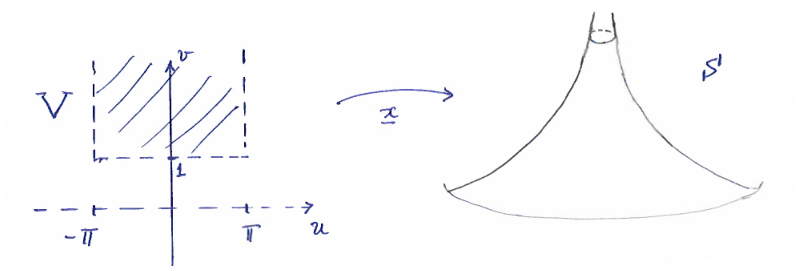
\includegraphics[height=0.7\textheight, width=0.7\textwidth, keepaspectratio]{./Images/hyperbolic_plane_11.png}
		\end{center}
	\end{figure}
	Suponha que temos os seguintes coeficientes da primeira forma fundamental:
	\[
		E = \frac{1}{v^{2}},\; F = 0,\; \& \; G = \frac{1}{v^{2}},
	\]
	e considere a curva \(\alpha (t) = \underline{x}(0, t),\; v_{0}\leq t \leq v\), ou seja, que o traço da curva é a imagem por \(\underline{x}\) do segmento vertical \(u=0\) entre \(v_{0}\) e v.
	Então, o comprimento da curva \(\alpha \) em S é dado por
	\begin{align*}
		\ell (\alpha ) = \int_{v_{0}}^{v}\Vert \alpha '(t) \Vert \mathrm{d}t & = \int_{v0}^{v}[(u')^{2}E + 2u'v'F + (v')^{2}G]^{\frac{1}{2}} \mathrm{d}t \\
		                                                                     & = \int_{v_{0}}^{v}\sqrt[]{\frac{1}{t^{2}}} \mathrm{d}t                    \\
		                                                                     & = \int_{v_{0}}^{v}\frac{1}{t} \mathrm{d}t                                 \\
		                                                                     & = \ln^{}{\biggl(\frac{v}{v_{0}}\biggr)},
	\end{align*}
	e, em particular, conforme \(v_{0}\) se aproxima de 0, o limite do comprimento da curva tende ao infinito!

	[Continua na próxima aula...]
\end{example}

\end{document}

